
\begin{minipage}[t]{0.6\textwidth}
On considère une fonction $f$ définie et dérivable sur l'intervalle $[-2~;~6]$. \\
Sa courbe représentative, notée $C$, est donnée ci-contre.

\begin{itemize}
\item On sait que la courbe $C$ passe par les points de coordonnées $(0~;~8)$, $(2~;~0)$ et $(4~;~-8)$.
\item On note $T$ la tangente à la courbe $C$ au point d'abscisse $x = 2$.
\item On sait que la tangente $T$ coupe l'axe des ordonnées en $y = 12$.
\end{itemize}

On note $f'$ la fonction dérivée de $f$.
\end{minipage}
\hfill
\begin{minipage}[t]{0.35\textwidth}
\vspace{0pt}
\begin{center}
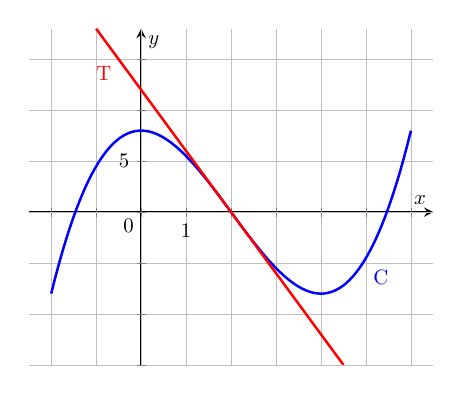
\begin{tikzpicture}[scale=0.75, transform shape]
  \begin{axis}[
    xmin=-2.5, xmax=6.5,
    ymin=-15, ymax=18,
    samples=100,
    axis lines=middle,
    xlabel=\(x\),
    ylabel=\(y\),
    ytick={5},
    xtick={1},
    extra y ticks={-15,-10,-5,0,10,15},
    extra x ticks={-2,-1,0,2,3,4,5,6},
    extra tick style={tick label style={opacity=0}},
    grid=both,
    grid style={line width=.1pt, draw=gray!10},
    major grid style={line width=.2pt,draw=gray!50},
    axis line style={line width=1pt},
    xtick distance=1,
    ytick distance=5,
    xmajorgrids,
    ymajorgrids,
    restrict y to domain=-15:18,
    restrict x to domain=-2.5:6.5,
  ]

  \node[below left] at (axis cs:0,0) {0};
  \node[blue, below right] at (axis cs:5,-5) {C};
  \addplot[blue, very thick, domain=-2:6] {0.5*x^3 - 3*x^2 + 8};
  \node[red, below left] at (axis cs:-0.5,15) {T};
  \addplot[red, very thick, domain=-1:4.5] {-6*x + 12};
  \end{axis}
\end{tikzpicture}
\end{center}
\end{minipage}

\begin{enumerate}
\item 
\begin{enumerate}
\item Déterminer les valeurs de $f(2)$ et $f'(2)$.
\item Donner une équation de la tangente $T$.
\item Recopier et compléter le tableau de variation ci-dessous en utilisant le graphique.

\begin{center}
\setlength{\tabcolsep}{18pt}
\begin{tabular}{|c|cccc|}
\hline
$x$ & $-2$ & $0$ & $4$ & $6$ \\
\hline
 & & & & \\
Variations & & & & \\
de $f$ & & & & \\
 & & & & \\
\hline
\end{tabular}
\end{center}
\end{enumerate}

\item On admet que la fonction $f$ est définie sur l'intervalle $[-2~;~6]$ par $f(x) = 0,5x^3 - 3x^2 + 8$.
\begin{enumerate}
\item Montrer que, pour tout réel $x$ de l'intervalle $[-2~;~6]$, on a $f'(x) = 1,5x(x - 4)$.
\item Étudier le signe de $f'(x)$ et retrouver le tableau de variation de la fonction $f$ sur l'intervalle $[-2~;~6]$.
\end{enumerate}

\item On admet que, pour tout réel $x$ de l'intervalle $[0~;~2]$, on a $f(x) \leq -6x + 12$. \\
Que peut-on en déduire pour la courbe $C$ et la tangente $T$ sur l'intervalle $[0~;~2]$ ?
\end{enumerate}




